\documentclass[11pt,compress,t,notes=noshow, xcolor=table]{beamer}
\usepackage[]{graphicx}\usepackage[]{color}
% maxwidth is the original width if it is less than linewidth
% otherwise use linewidth (to make sure the graphics do not exceed the margin)
\makeatletter
\def\maxwidth{ %
  \ifdim\Gin@nat@width>\linewidth
    \linewidth
  \else
    \Gin@nat@width
  \fi
}
\makeatother

\newcommand{\citebutton}[2]{%
\beamergotobutton{\href{#2}{#1}}%
}

\newcommand{\blu}[1]{\textcolor{blue}{#1}}
\newcommand{\org}[1]{\textcolor{orange}{#1}}
\newcommand{\ques}{\textbf{\textcolor{red}{Question:  }}}
\newcommand{\questionssofar}{\begin{frame}\frametitle{Any questions?}\end{frame}}

\newcommand\warning{%
 \makebox[1.4em][c]{%
 \makebox[0pt][c]{\raisebox{.1em}{\scriptsize!}}%
 \makebox[0pt][c]{\color{red}\normalsize$\bigtriangleup$}}}%

\definecolor{fgcolor}{rgb}{0.345, 0.345, 0.345}
\newcommand{\hlnum}[1]{\textcolor[rgb]{0.686,0.059,0.569}{#1}}%
\newcommand{\hlstr}[1]{\textcolor[rgb]{0.192,0.494,0.8}{#1}}%
\newcommand{\hlcom}[1]{\textcolor[rgb]{0.678,0.584,0.686}{\textit{#1}}}%
\newcommand{\hlopt}[1]{\textcolor[rgb]{0,0,0}{#1}}%
\newcommand{\hlstd}[1]{\textcolor[rgb]{0.345,0.345,0.345}{#1}}%
\newcommand{\hlkwa}[1]{\textcolor[rgb]{0.161,0.373,0.58}{\textbf{#1}}}%
\newcommand{\hlkwb}[1]{\textcolor[rgb]{0.69,0.353,0.396}{#1}}%
\newcommand{\hlkwc}[1]{\textcolor[rgb]{0.333,0.667,0.333}{#1}}%
\newcommand{\hlkwd}[1]{\textcolor[rgb]{0.737,0.353,0.396}{\textbf{#1}}}%
\let\hlipl\hlkwb

\usepackage{framed}
\makeatletter
\newenvironment{kframe}{%
 \def\at@end@of@kframe{}%
 \ifinner\ifhmode%
  \def\at@end@of@kframe{\end{minipage}}%
  \begin{minipage}{\columnwidth}%
 \fi\fi%
 \def\FrameCommand##1{\hskip\@totalleftmargin \hskip-\fboxsep
 \colorbox{shadecolor}{##1}\hskip-\fboxsep
     % There is no \\@totalrightmargin, so:
     \hskip-\linewidth \hskip-\@totalleftmargin \hskip\columnwidth}%
 \MakeFramed {\advance\hsize-\width
   \@totalleftmargin\z@ \linewidth\hsize
   \@setminipage}}%
 {\par\unskip\endMakeFramed%
 \at@end@of@kframe}
\makeatother

\definecolor{shadecolor}{rgb}{.97, .97, .97}
\definecolor{messagecolor}{rgb}{0, 0, 0}
\definecolor{warningcolor}{rgb}{1, 0, 1}
\definecolor{errorcolor}{rgb}{1, 0, 0}
\newenvironment{knitrout}{}{} % an empty environment to be redefined in TeX

\usepackage{alltt}
\newcommand{\SweaveOpts}[1]{}  % do not interfere with LaTeX
\newcommand{\SweaveInput}[1]{} % because they are not real TeX commands
\newcommand{\Sexpr}[1]{}       % will only be parsed by R
\newcommand{\xmark}{\ding{55}}%


\usepackage[english]{babel}
\usepackage[utf8]{inputenc}

\usepackage{dsfont}
\usepackage{verbatim}
\usepackage{amsmath}
\usepackage{amsfonts}
\usepackage{amssymb}
\usepackage{bm}
\usepackage{csquotes}
\usepackage{multirow}
\usepackage{longtable}
\usepackage{booktabs}
\usepackage{enumerate}
\usepackage[absolute,overlay]{textpos}
\usepackage{psfrag}
\usepackage{algorithm}
\usepackage{algpseudocode}
\usepackage{eqnarray}
\usepackage{arydshln}
\usepackage{tabularx}
\usepackage{placeins}
\usepackage{tikz}
\usepackage{setspace}
\usepackage{colortbl}
\usepackage{mathtools}
\usepackage{wrapfig}
\usepackage{bm}
\usepackage{amsmath}
\usepackage{pifont}

\usetikzlibrary{shapes.multipart,shapes,arrows,automata,positioning,calc,chains,trees, shadows}
\tikzset{
  %Define standard arrow tip
  >=stealth',
  %Define style for boxes
  punkt/.style={
    rectangle,
    rounded corners,
    draw=black, very thick,
    text width=6.5em,
    minimum height=2em,
    text centered},
  % Define arrow style
  pil/.style={
    ->,
    thick,
    shorten <=2pt,
    shorten >=2pt,}
}

\tikzstyle{vec}=[draw, rectangle, fill = white, minimum width=5mm, minimum height=1cm, inner sep = 2pt]

\usepackage{subfig}

% Defines macros and environments
\usepackage{../../style/lmu-lecture}


\let\code=\texttt
\let\proglang=\textsf

\setkeys{Gin}{width=0.9\textwidth}

\setbeamertemplate{frametitle}{\expandafter\uppercase\expandafter\insertframetitle}

\usepackage{bbm}
% basic latex stuff
\newcommand{\pkg}[1]{{\fontseries{b}\selectfont #1}} %fontstyle for R packages
\newcommand{\lz}{\vspace{0.5cm}} %vertical space
\newcommand{\dlz}{\vspace{1cm}} %double vertical space
\newcommand{\oneliner}[1] % Oneliner for important statements
{\begin{block}{}\begin{center}\begin{Large}#1\end{Large}\end{center}\end{block}}


%new environments
\newenvironment{vbframe}  %frame with breaks and verbatim
{
 \begin{frame}[containsverbatim,allowframebreaks]
}
{
\end{frame}
}

\newenvironment{vframe}  %frame with verbatim without breaks (to avoid numbering one slided frames)
{
 \begin{frame}[containsverbatim]
}
{
\end{frame}
}

\newenvironment{blocki}[1]   % itemize block
{
 \begin{block}{#1}\begin{itemize}
}
{
\end{itemize}\end{block}
}

\newenvironment{fragileframe}[2]{  %fragile frame with framebreaks
\begin{frame}[allowframebreaks, fragile, environment = fragileframe]
\frametitle{#1}
#2}
{\end{frame}}


\newcommand{\myframe}[2]{  %short for frame with framebreaks
\begin{frame}[allowframebreaks]
\frametitle{#1}
#2
\end{frame}}

\newcommand{\remark}[1]{
  \textbf{Remark:} #1
}


\newenvironment{deleteframe}
{
\begingroup
\usebackgroundtemplate{
\includegraphics[width=\paperwidth,height=\paperheight]{../style/color/red.png}}
 \begin{frame}
}
{
\end{frame}
\endgroup
}
\newenvironment{simplifyframe}
{
\begingroup
\usebackgroundtemplate{
\includegraphics[width=\paperwidth,height=\paperheight]{../style/color/yellow.png}}
 \begin{frame}
}
{
\end{frame}
\endgroup
}\newenvironment{draftframe}
{
\begingroup
\usebackgroundtemplate{
\includegraphics[width=\paperwidth,height=\paperheight]{../style/color/green.jpg}}
 \begin{frame}
}
{
\end{frame}
\endgroup
}
% https://tex.stackexchange.com/a/261480: textcolor that works in mathmode
\makeatletter
\renewcommand*{\@textcolor}[3]{%
  \protect\leavevmode
  \begingroup
    \color#1{#2}#3%
  \endgroup
}
\makeatother





% math spaces
\ifdefined\N                                                                
\renewcommand{\N}{\mathds{N}} % N, naturals
\else \newcommand{\N}{\mathds{N}} \fi 
\newcommand{\Z}{\mathds{Z}} % Z, integers
\newcommand{\Q}{\mathds{Q}} % Q, rationals
\newcommand{\R}{\mathds{R}} % R, reals
\ifdefined\C 
  \renewcommand{\C}{\mathds{C}} % C, complex
\else \newcommand{\C}{\mathds{C}} \fi
\newcommand{\continuous}{\mathcal{C}} % C, space of continuous functions
\newcommand{\M}{\mathcal{M}} % machine numbers
\newcommand{\epsm}{\epsilon_m} % maximum error

% counting / finite sets
\newcommand{\setzo}{\{0, 1\}} % set 0, 1
\newcommand{\setmp}{\{-1, +1\}} % set -1, 1
\newcommand{\unitint}{[0, 1]} % unit interval

% basic math stuff
\newcommand{\xt}{\tilde x} % x tilde
\newcommand{\argmax}{\operatorname{arg\,max}} % argmax
\newcommand{\argmin}{\operatorname{arg\,min}} % argmin
\newcommand{\argminlim}{\mathop{\mathrm{arg\,min}}\limits} % argmax with limits
\newcommand{\argmaxlim}{\mathop{\mathrm{arg\,max}}\limits} % argmin with limits  
\newcommand{\sign}{\operatorname{sign}} % sign, signum
\newcommand{\I}{\mathbb{I}} % I, indicator
\newcommand{\order}{\mathcal{O}} % O, order
\newcommand{\pd}[2]{\frac{\partial{#1}}{\partial #2}} % partial derivative
\newcommand{\floorlr}[1]{\left\lfloor #1 \right\rfloor} % floor
\newcommand{\ceillr}[1]{\left\lceil #1 \right\rceil} % ceiling

% sums and products
\newcommand{\sumin}{\sum\limits_{i=1}^n} % summation from i=1 to n
\newcommand{\sumim}{\sum\limits_{i=1}^m} % summation from i=1 to m
\newcommand{\sumjn}{\sum\limits_{j=1}^n} % summation from j=1 to p
\newcommand{\sumjp}{\sum\limits_{j=1}^p} % summation from j=1 to p
\newcommand{\sumik}{\sum\limits_{i=1}^k} % summation from i=1 to k
\newcommand{\sumkg}{\sum\limits_{k=1}^g} % summation from k=1 to g
\newcommand{\sumjg}{\sum\limits_{j=1}^g} % summation from j=1 to g
\newcommand{\meanin}{\frac{1}{n} \sum\limits_{i=1}^n} % mean from i=1 to n
\newcommand{\meanim}{\frac{1}{m} \sum\limits_{i=1}^m} % mean from i=1 to n
\newcommand{\meankg}{\frac{1}{g} \sum\limits_{k=1}^g} % mean from k=1 to g
\newcommand{\prodin}{\prod\limits_{i=1}^n} % product from i=1 to n
\newcommand{\prodkg}{\prod\limits_{k=1}^g} % product from k=1 to g
\newcommand{\prodjp}{\prod\limits_{j=1}^p} % product from j=1 to p

% linear algebra
\newcommand{\one}{\boldsymbol{1}} % 1, unitvector
\newcommand{\zero}{\mathbf{0}} % 0-vector
\newcommand{\id}{\boldsymbol{I}} % I, identity
\newcommand{\diag}{\operatorname{diag}} % diag, diagonal
\newcommand{\trace}{\operatorname{tr}} % tr, trace
\newcommand{\spn}{\operatorname{span}} % span
\newcommand{\scp}[2]{\left\langle #1, #2 \right\rangle} % <.,.>, scalarproduct
\newcommand{\mat}[1]{\begin{pmatrix} #1 \end{pmatrix}} % short pmatrix command
\newcommand{\Amat}{\mathbf{A}} % matrix A
\newcommand{\Deltab}{\mathbf{\Delta}} % error term for vectors

% basic probability + stats
\renewcommand{\P}{\mathds{P}} % P, probability
\newcommand{\E}{\mathds{E}} % E, expectation
\newcommand{\var}{\mathsf{Var}} % Var, variance
\newcommand{\cov}{\mathsf{Cov}} % Cov, covariance
\newcommand{\corr}{\mathsf{Corr}} % Corr, correlation
\newcommand{\normal}{\mathcal{N}} % N of the normal distribution
\newcommand{\iid}{\overset{i.i.d}{\sim}} % dist with i.i.d superscript
\newcommand{\distas}[1]{\overset{#1}{\sim}} % ... is distributed as ...

% machine learning
\newcommand{\Xspace}{\mathcal{X}} % X, input space
\newcommand{\Yspace}{\mathcal{Y}} % Y, output space
\newcommand{\nset}{\{1, \ldots, n\}} % set from 1 to n
\newcommand{\pset}{\{1, \ldots, p\}} % set from 1 to p
\newcommand{\gset}{\{1, \ldots, g\}} % set from 1 to g
\newcommand{\Pxy}{\mathbb{P}_{xy}} % P_xy
\newcommand{\Exy}{\mathbb{E}_{xy}} % E_xy: Expectation over random variables xy
\newcommand{\xv}{\mathbf{x}} % vector x (bold)
\newcommand{\xtil}{\tilde{\mathbf{x}}} % vector x-tilde (bold)
\newcommand{\yv}{\mathbf{y}} % vector y (bold)
\newcommand{\xy}{(\xv, y)} % observation (x, y)
\newcommand{\xvec}{\left(x_1, \ldots, x_p\right)^\top} % (x1, ..., xp) 
\newcommand{\Xmat}{\mathbf{X}} % Design matrix
\newcommand{\allDatasets}{\mathds{D}} % The set of all datasets
\newcommand{\allDatasetsn}{\mathds{D}_n}  % The set of all datasets of size n 
\newcommand{\D}{\mathcal{D}} % D, data
\newcommand{\Dn}{\D_n} % D_n, data of size n
\newcommand{\Dtrain}{\mathcal{D}_{\text{train}}} % D_train, training set
\newcommand{\Dtest}{\mathcal{D}_{\text{test}}} % D_test, test set
\newcommand{\xyi}[1][i]{\left(\xv^{(#1)}, y^{(#1)}\right)} % (x^i, y^i), i-th observation
\newcommand{\Dset}{\left( \xyi[1], \ldots, \xyi[n]\right)} % {(x1,y1)), ..., (xn,yn)}, data
\newcommand{\defAllDatasetsn}{(\Xspace \times \Yspace)^n} % Def. of the set of all datasets of size n 
\newcommand{\defAllDatasets}{\bigcup_{n \in \N}(\Xspace \times \Yspace)^n} % Def. of the set of all datasets 
\newcommand{\xdat}{\left\{ \xv^{(1)}, \ldots, \xv^{(n)}\right\}} % {x1, ..., xn}, input data
\newcommand{\yvec}{\left(y^{(1)}, \hdots, y^{(n)}\right)^\top} % (y1, ..., yn), vector of outcomes
\renewcommand{\xi}[1][i]{\xv^{(#1)}} % x^i, i-th observed value of x
\newcommand{\yi}[1][i]{y^{(#1)}} % y^i, i-th observed value of y 
\newcommand{\xivec}{\left(x^{(i)}_1, \ldots, x^{(i)}_p\right)^\top} % (x1^i, ..., xp^i), i-th observation vector
\newcommand{\xj}{\xv_j} % x_j, j-th feature
\newcommand{\xjvec}{\left(x^{(1)}_j, \ldots, x^{(n)}_j\right)^\top} % (x^1_j, ..., x^n_j), j-th feature vector
\newcommand{\phiv}{\mathbf{\phi}} % Basis transformation function phi
\newcommand{\phixi}{\mathbf{\phi}^{(i)}} % Basis transformation of xi: phi^i := phi(xi)

%%%%%% ml - models general
\newcommand{\lamv}{\bm{\lambda}} % lambda vector, hyperconfiguration vector
\newcommand{\Lam}{\bm{\Lambda}}	 % Lambda, space of all hpos
% Inducer / Inducing algorithm
\newcommand{\preimageInducer}{\left(\defAllDatasets\right)\times\Lam} % Set of all datasets times the hyperparameter space
\newcommand{\preimageInducerShort}{\allDatasets\times\Lam} % Set of all datasets times the hyperparameter space
% Inducer / Inducing algorithm
\newcommand{\ind}{\mathcal{I}} % Inducer, inducing algorithm, learning algorithm 

% continuous prediction function f
\newcommand{\ftrue}{f_{\text{true}}}  % True underlying function (if a statistical model is assumed)
\newcommand{\ftruex}{\ftrue(\xv)} % True underlying function (if a statistical model is assumed)
\newcommand{\fx}{f(\xv)} % f(x), continuous prediction function
\newcommand{\fdomains}{f: \Xspace \rightarrow \R^g} % f with domain and co-domain
\newcommand{\Hspace}{\mathcal{H}} % hypothesis space where f is from
\newcommand{\fbayes}{f^{\ast}} % Bayes-optimal model
\newcommand{\fxbayes}{f^{\ast}(\xv)} % Bayes-optimal model
\newcommand{\fkx}[1][k]{f_{#1}(\xv)} % f_j(x), discriminant component function
\newcommand{\fh}{\hat{f}} % f hat, estimated prediction function
\newcommand{\fxh}{\fh(\xv)} % fhat(x)
\newcommand{\fxt}{f(\xv ~|~ \thetab)} % f(x | theta)
\newcommand{\fxi}{f\left(\xv^{(i)}\right)} % f(x^(i))
\newcommand{\fxih}{\hat{f}\left(\xv^{(i)}\right)} % f(x^(i))
\newcommand{\fxit}{f\left(\xv^{(i)} ~|~ \thetab\right)} % f(x^(i) | theta)
\newcommand{\fhD}{\fh_{\D}} % fhat_D, estimate of f based on D
\newcommand{\fhDtrain}{\fh_{\Dtrain}} % fhat_Dtrain, estimate of f based on D
\newcommand{\fhDnlam}{\fh_{\Dn, \lamv}} %model learned on Dn with hp lambda
\newcommand{\fhDlam}{\fh_{\D, \lamv}} %model learned on D with hp lambda
\newcommand{\fhDnlams}{\fh_{\Dn, \lamv^\ast}} %model learned on Dn with optimal hp lambda 
\newcommand{\fhDlams}{\fh_{\D, \lamv^\ast}} %model learned on D with optimal hp lambda 

% discrete prediction function h
\newcommand{\hx}{h(\xv)} % h(x), discrete prediction function
\newcommand{\hh}{\hat{h}} % h hat
\newcommand{\hxh}{\hat{h}(\xv)} % hhat(x)
\newcommand{\hxt}{h(\xv | \thetab)} % h(x | theta)
\newcommand{\hxi}{h\left(\xi\right)} % h(x^(i))
\newcommand{\hxit}{h\left(\xi ~|~ \thetab\right)} % h(x^(i) | theta)
\newcommand{\hbayes}{h^{\ast}} % Bayes-optimal classification model
\newcommand{\hxbayes}{h^{\ast}(\xv)} % Bayes-optimal classification model

% yhat
\newcommand{\yh}{\hat{y}} % yhat for prediction of target
\newcommand{\yih}{\hat{y}^{(i)}} % yhat^(i) for prediction of ith targiet
\newcommand{\resi}{\yi- \yih}

% theta
\newcommand{\thetah}{\hat{\theta}} % theta hat
\newcommand{\thetab}{\bm{\theta}} % theta vector
\newcommand{\thetabh}{\bm{\hat\theta}} % theta vector hat
\newcommand{\thetat}[1][t]{\thetab^{[#1]}} % theta^[t] in optimization
\newcommand{\thetatn}[1][t]{\thetab^{[#1 +1]}} % theta^[t+1] in optimization
\newcommand{\thetahDnlam}{\thetabh_{\Dn, \lamv}} %theta learned on Dn with hp lambda
\newcommand{\thetahDlam}{\thetabh_{\D, \lamv}} %theta learned on D with hp lambda
\newcommand{\mint}{\min_{\thetab \in \Theta}} % min problem theta
\newcommand{\argmint}{\argmin_{\thetab \in \Theta}} % argmin theta

% densities + probabilities
% pdf of x 
\newcommand{\pdf}{p} % p
\newcommand{\pdfx}{p(\xv)} % p(x)
\newcommand{\pixt}{\pi(\xv~|~ \thetab)} % pi(x|theta), pdf of x given theta
\newcommand{\pixit}{\pi\left(\xi ~|~ \thetab\right)} % pi(x^i|theta), pdf of x given theta
\newcommand{\pixii}{\pi\left(\xi\right)} % pi(x^i), pdf of i-th x 

% pdf of (x, y)
\newcommand{\pdfxy}{p(\xv,y)} % p(x, y)
\newcommand{\pdfxyt}{p(\xv, y ~|~ \thetab)} % p(x, y | theta)
\newcommand{\pdfxyit}{p\left(\xi, \yi ~|~ \thetab\right)} % p(x^(i), y^(i) | theta)

% pdf of x given y
\newcommand{\pdfxyk}[1][k]{p(\xv | y= #1)} % p(x | y = k)
\newcommand{\lpdfxyk}[1][k]{\log p(\xv | y= #1)} % log p(x | y = k)
\newcommand{\pdfxiyk}[1][k]{p\left(\xi | y= #1 \right)} % p(x^i | y = k)

% prior probabilities
\newcommand{\pik}[1][k]{\pi_{#1}} % pi_k, prior
\newcommand{\lpik}[1][k]{\log \pi_{#1}} % log pi_k, log of the prior
\newcommand{\pit}{\pi(\thetab)} % Prior probability of parameter theta

% posterior probabilities
\newcommand{\post}{\P(y = 1 ~|~ \xv)} % P(y = 1 | x), post. prob for y=1
\newcommand{\postk}[1][k]{\P(y = #1 ~|~ \xv)} % P(y = k | y), post. prob for y=k
\newcommand{\pidomains}{\pi: \Xspace \rightarrow \unitint} % pi with domain and co-domain
\newcommand{\pibayes}{\pi^{\ast}} % Bayes-optimal classification model
\newcommand{\pixbayes}{\pi^{\ast}(\xv)} % Bayes-optimal classification model
\newcommand{\pix}{\pi(\xv)} % pi(x), P(y = 1 | x)
\newcommand{\pikx}[1][k]{\pi_{#1}(\xv)} % pi_k(x), P(y = k | x)
\newcommand{\pikxt}[1][k]{\pi_{#1}(\xv ~|~ \thetab)} % pi_k(x | theta), P(y = k | x, theta)
\newcommand{\pixh}{\hat \pi(\xv)} % pi(x) hat, P(y = 1 | x) hat
\newcommand{\pikxh}[1][k]{\hat \pi_{#1}(\xv)} % pi_k(x) hat, P(y = k | x) hat
\newcommand{\pixih}{\hat \pi(\xi)} % pi(x^(i)) with hat
\newcommand{\pikxih}[1][k]{\hat \pi_{#1}(\xi)} % pi_k(x^(i)) with hat
\newcommand{\pdfygxt}{p(y ~|~\xv, \thetab)} % p(y | x, theta)
\newcommand{\pdfyigxit}{p\left(\yi ~|~\xi, \thetab\right)} % p(y^i |x^i, theta)
\newcommand{\lpdfygxt}{\log \pdfygxt } % log p(y | x, theta)
\newcommand{\lpdfyigxit}{\log \pdfyigxit} % log p(y^i |x^i, theta)

% probababilistic
\newcommand{\bayesrulek}[1][k]{\frac{\P(\xv | y= #1) \P(y= #1)}{\P(\xv)}} % Bayes rule
\newcommand{\muk}{\bm{\mu_k}} % mean vector of class-k Gaussian (discr analysis) 

% residual and margin
\newcommand{\eps}{\epsilon} % residual, stochastic
\newcommand{\epsi}{\epsilon^{(i)}} % epsilon^i, residual, stochastic
\newcommand{\epsh}{\hat{\epsilon}} % residual, estimated
\newcommand{\yf}{y \fx} % y f(x), margin
\newcommand{\yfi}{\yi \fxi} % y^i f(x^i), margin
\newcommand{\Sigmah}{\hat \Sigma} % estimated covariance matrix
\newcommand{\Sigmahj}{\hat \Sigma_j} % estimated covariance matrix for the j-th class

% ml - loss, risk, likelihood
\newcommand{\Lyf}{L\left(y, f\right)} % L(y, f), loss function
\newcommand{\Lxy}{L\left(y, \fx\right)} % L(y, f(x)), loss function
\newcommand{\Lxyi}{L\left(\yi, \fxi\right)} % loss of observation
\newcommand{\Lxyt}{L\left(y, \fxt\right)} % loss with f parameterized
\newcommand{\Lxyit}{L\left(\yi, \fxit\right)} % loss of observation with f parameterized
\newcommand{\Lxym}{L\left(\yi, f\left(\bm{\tilde{x}}^{(i)} ~|~ \thetab\right)\right)} % loss of observation with f parameterized
\newcommand{\Lpixy}{L\left(y, \pix\right)} % loss in classification
\newcommand{\Lpixyi}{L\left(\yi, \pixii\right)} % loss of observation in classification
\newcommand{\Lpixyt}{L\left(y, \pixt\right)} % loss with pi parameterized
\newcommand{\Lpixyit}{L\left(\yi, \pixit\right)} % loss of observation with pi parameterized
\newcommand{\Lhxy}{L\left(y, \hx\right)} % L(y, h(x)), loss function on discrete classes
\newcommand{\Lr}{L\left(r\right)} % L(r), loss defined on residual (reg) / margin (classif)
\newcommand{\lone}{|y - \fx|} % L1 loss
\newcommand{\ltwo}{\left(y - \fx\right)^2} % L2 loss
\newcommand{\lbernoullimp}{\ln(1 + \exp(-y \cdot \fx))} % Bernoulli loss for -1, +1 encoding
\newcommand{\lbernoullizo}{- y \cdot \fx + \log(1 + \exp(\fx))} % Bernoulli loss for 0, 1 encoding
\newcommand{\lcrossent}{- y \log \left(\pix\right) - (1 - y) \log \left(1 - \pix\right)} % cross-entropy loss
\newcommand{\lbrier}{\left(\pix - y \right)^2} % Brier score
\newcommand{\risk}{\mathcal{R}} % R, risk
\newcommand{\riskbayes}{\mathcal{R}^\ast}
\newcommand{\riskf}{\risk(f)} % R(f), risk
\newcommand{\riskdef}{\E_{y|\xv}\left(\Lxy \right)} % risk def (expected loss)
\newcommand{\riskt}{\mathcal{R}(\thetab)} % R(theta), risk
\newcommand{\riske}{\mathcal{R}_{\text{emp}}} % R_emp, empirical risk w/o factor 1 / n
\newcommand{\riskeb}{\bar{\mathcal{R}}_{\text{emp}}} % R_emp, empirical risk w/ factor 1 / n
\newcommand{\riskef}{\riske(f)} % R_emp(f)
\newcommand{\risket}{\mathcal{R}_{\text{emp}}(\thetab)} % R_emp(theta)
\newcommand{\riskr}{\mathcal{R}_{\text{reg}}} % R_reg, regularized risk
\newcommand{\riskrt}{\mathcal{R}_{\text{reg}}(\thetab)} % R_reg(theta)
\newcommand{\riskrf}{\riskr(f)} % R_reg(f)
\newcommand{\riskrth}{\hat{\mathcal{R}}_{\text{reg}}(\thetab)} % hat R_reg(theta)
\newcommand{\risketh}{\hat{\mathcal{R}}_{\text{emp}}(\thetab)} % hat R_emp(theta)
\newcommand{\LL}{\mathcal{L}} % L, likelihood
\newcommand{\LLt}{\mathcal{L}(\thetab)} % L(theta), likelihood
\newcommand{\LLtx}{\mathcal{L}(\thetab | \xv)} % L(theta|x), likelihood
\newcommand{\logl}{\ell} % l, log-likelihood
\newcommand{\loglt}{\logl(\thetab)} % l(theta), log-likelihood
\newcommand{\logltx}{\logl(\thetab | \xv)} % l(theta|x), log-likelihood
\newcommand{\errtrain}{\text{err}_{\text{train}}} % training error
\newcommand{\errtest}{\text{err}_{\text{test}}} % test error
\newcommand{\errexp}{\overline{\text{err}_{\text{test}}}} % avg training error

% lm
\newcommand{\thx}{\thetab^\top \xv} % linear model
\newcommand{\olsest}{(\Xmat^\top \Xmat)^{-1} \Xmat^\top \yv} % OLS estimator in LM 

\usepackage{movie15}
\usepackage{animate}

\newcommand{\titlefigure}{figure/sesamestreet.jpeg}
\newcommand{\learninggoals}{
\item shortcomings of BERT \& Co.
\item everything as text-to-text
\item Dynamic Masking}

\title{Using the Transformer}
% \author{}
\institute{\href{https://slds-lmu.github.io/lecture_dl4nlp/}{slds-lmu.github.io/lecture\_dl4nlp}}
\date{}

\begin{document}
\lecturechapter{Text-to-Text Transfer Transformer}
\lecture{Deep Learning for NLP}

% ------------------------------------------------------------------------------

\begin{frame}{Revisiting text-to-text tasks}

\vfill
	
	\begin{figure}
		\centering
		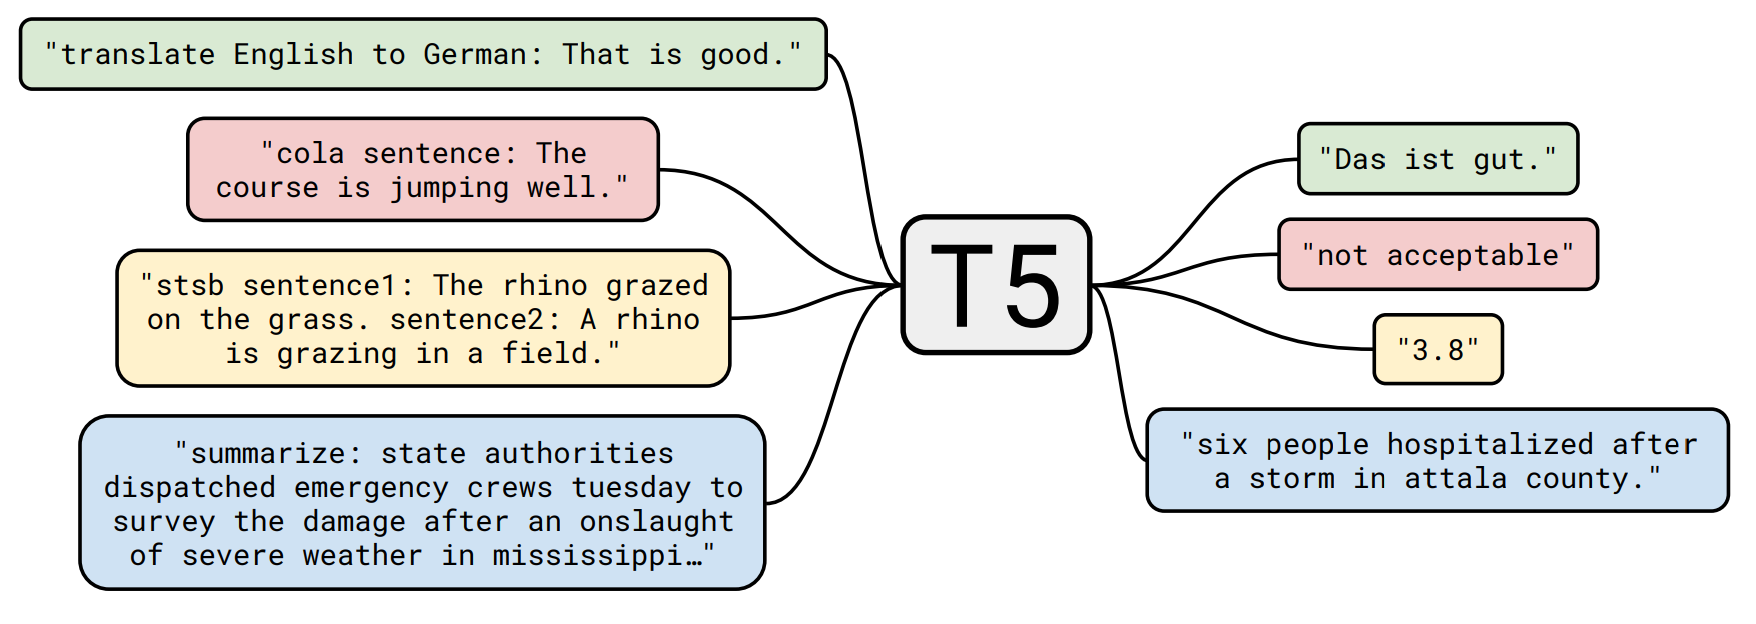
\includegraphics[width = 11cm]{figure/62-t5.png}\\ 
		\citebutton{Source: Raffel et al., 2020}{https://jmlr.org/papers/v21/20-074.html}
	\end{figure}
	
\textbf{Ingredients:}
	
\begin{itemize}
	\item \texttt{<task prefix>} for each task
	\item[] $\to$ Concatenation with the input
	\item Output label / score formatted as string
\end{itemize}
	
\vfill

\end{frame}

% ------------------------------------------------------------------------------

\begin{frame}{Text-to-Text Transfer Transformer}

\vfill

	\textbf{Short summary:}

	\begin{itemize}
		\item In short: T5 (bc of the five Ts)
		\item A complete encoder-decoder Transformer architecture
		\item[] \ques Why is this important?
		\item Relative positional embeddings
		\item All tasks reformulated as text-to-text tasks
		\item[] $\to$ Probably the most important innovation of this work
		\item From BERT-size $\times2$ (since enc-dec) up to 11B parameters
		\item Paradigm shift from \textit{Sequential Transfer Learning} towards true \textit{Multi-Task Learning}
	\end{itemize}
	
	\vspace{.5cm}

	\begin{center}
		\href{https://1.bp.blogspot.com/-o4oiOExxq1s/Xk26XPC3haI/AAAAAAAAFU8/NBlvOWB84L0PTYy9TzZBaLf6fwPGJTR0QCLcBGAsYHQ/s1600/image3.gif}{\textbf{\beamergotobutton{Nice Animation (similar to figure before)}}}
	\end{center}
	
\vfill

\end{frame}

% ------------------------------------------------------------------------------

\begin{frame}{input and output format}

\vfill

	\textbf{Input Side:}

	\begin{itemize}
		\item SentencePiece framework w/ WordPiece tokens
		\item Add task-specific (text) prefix to the original input
		\item Choice of the prefix: Hyperparameter!! 
		\item[$\to$] Changing this had limited impact
		\item[$\to$] No extensive experiments performed by the authors
	\end{itemize}
	
	\vspace{.5cm}

	\textbf{Output Side:}

	\begin{itemize}
		\item Output as a word or a piece of text (also numerical similarity scores)
		\item If output not present in set of potential alternatives, prediction considered as wrong (many other possible ways; this is not trivial)
	\end{itemize}
	
\vfill

\end{frame}

% ------------------------------------------------------------------------------

\begin{frame}{task prefix vs. prompting}

\vfill

	\textbf{Adding task-specific (text) prefix:}

	\begin{itemize}
		\item Add task-specific (text) prefix to the original input
		\item Model is fine-tuned on samples prepended with this prefix
		\item[$\to$] It learns to recognize what it is expected to do when encountering a specific prefix at test time
		\item[$\to$] Probably because of this: limited impact found by the authors
	\end{itemize}
	
	\vspace{.5cm}

	\textbf{Prompting:}

	\begin{itemize}
		\item Refers to just querying a trained w/o fine-tuning it (cf. next chapter)
		\item Paradigm of Few-/Zero-Shot Learning
		\item This is found to have a \textit{huge} impact on model performance
	\end{itemize}
	
\vfill

\end{frame}

% ------------------------------------------------------------------------------

\begin{frame}{architectural differences}

\vfill
	
	\textbf{Attention patterns (top) and Schematics of considered architectures (bottom)}
	
	\begin{figure}
		\centering
		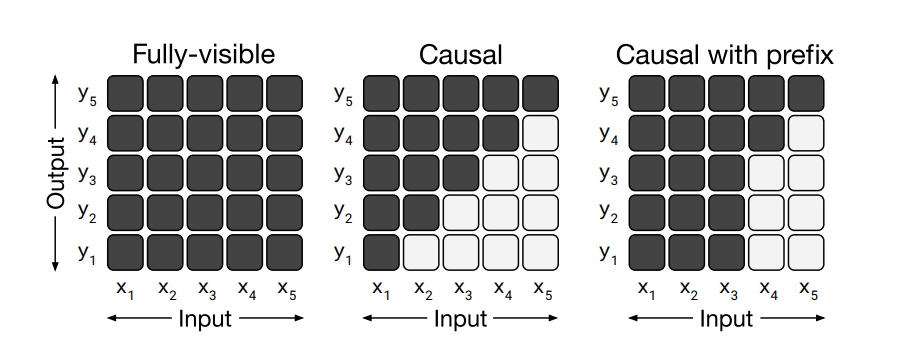
\includegraphics[width = 7.5cm]{figure/63-mask-patterns.png}\\ 
		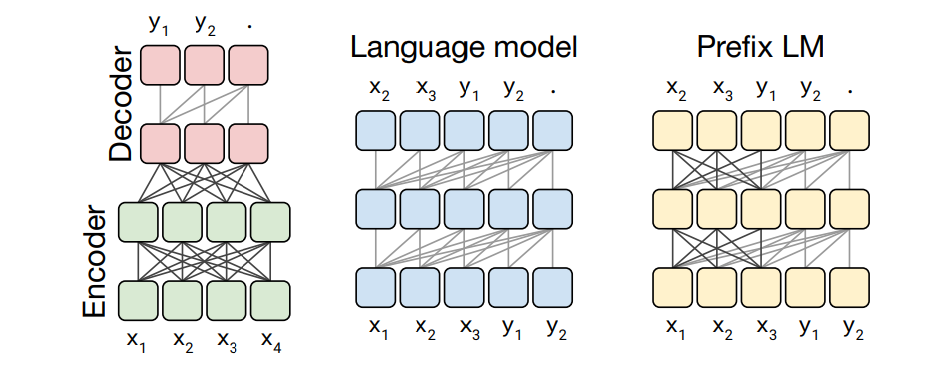
\includegraphics[width = 7.5cm]{figure/63-schematics.png}\\ 
		\citebutton{Source: Raffel et al., 2020}{https://jmlr.org/papers/v21/20-074.html}
	\end{figure}
	
\vfill

\end{frame}

% ------------------------------------------------------------------------------

\begin{frame}{pre-training objective}

\vfill
	
	\begin{figure}
		\centering
		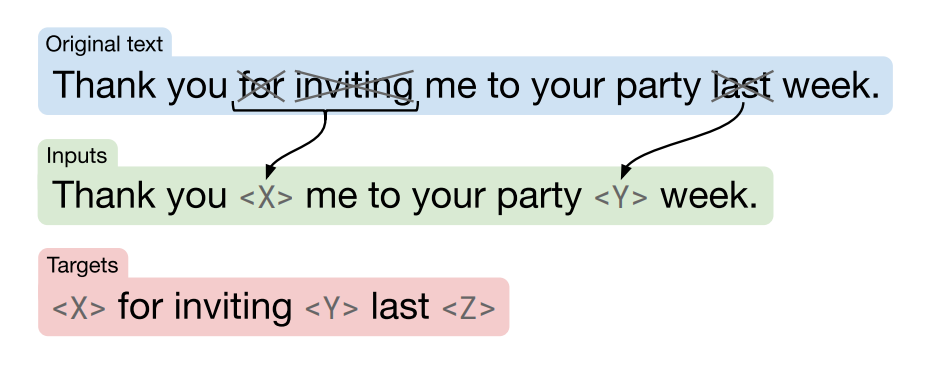
\includegraphics[width = 11cm]{figure/63-t5-span-pred.png}\\ 
		\citebutton{Source: Raffel et al., 2020}{https://jmlr.org/papers/v21/20-074.html}
	\end{figure}
	
	\begin{enumerate}
		\item Mark spans in input sequence for corruptions
		\item Replace tokens with sentinel tokens
		\item Predict sentinel tokens and replaced tokens
	\end{enumerate}
	
\vfill

\end{frame}

% ------------------------------------------------------------------------------

\begin{frame}{Pre-training objectives}

\vfill

	\begin{itemize}
		\item Authors experimented with different objectives
		\item Most of them rely in some way on MLM
	\end{itemize}
	
	\begin{figure}
		\centering
		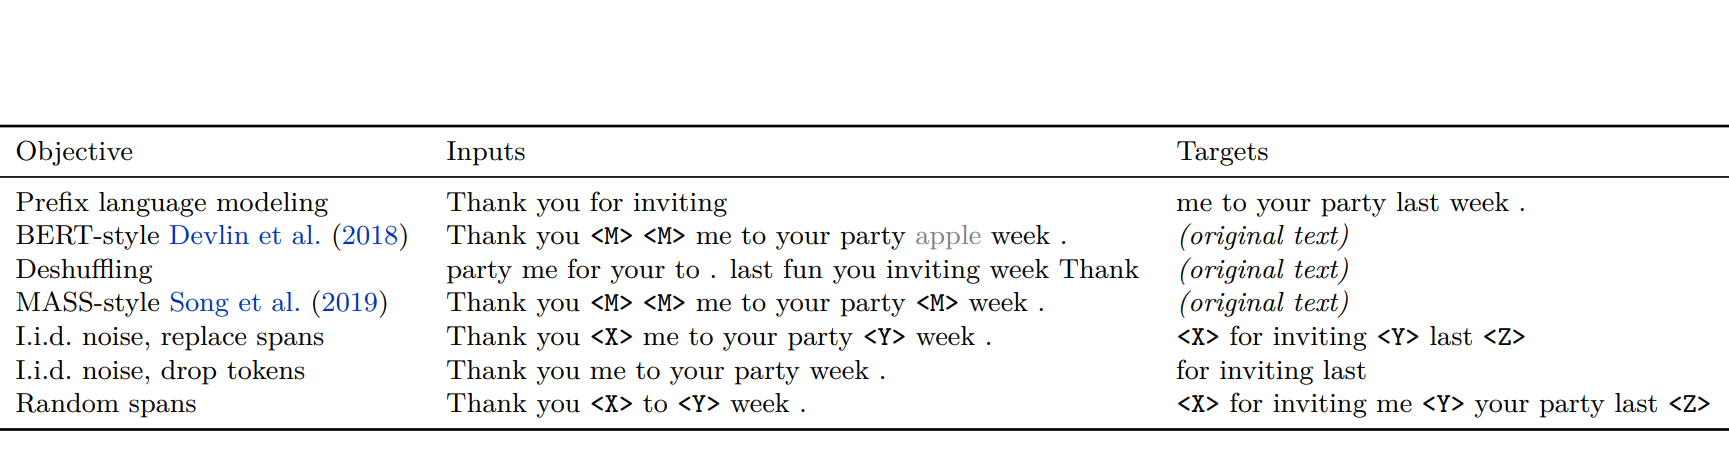
\includegraphics[width = 11cm]{figure/63-t5-objectives1.png}\\ 
		\citebutton{Source: Raffel et al., 2020}{https://jmlr.org/papers/v21/20-074.html}
	\end{figure}
	
\vfill

\end{frame}

% ------------------------------------------------------------------------------

\begin{frame}{Pre-training objectives}

\vfill

	\begin{figure}
		\centering
		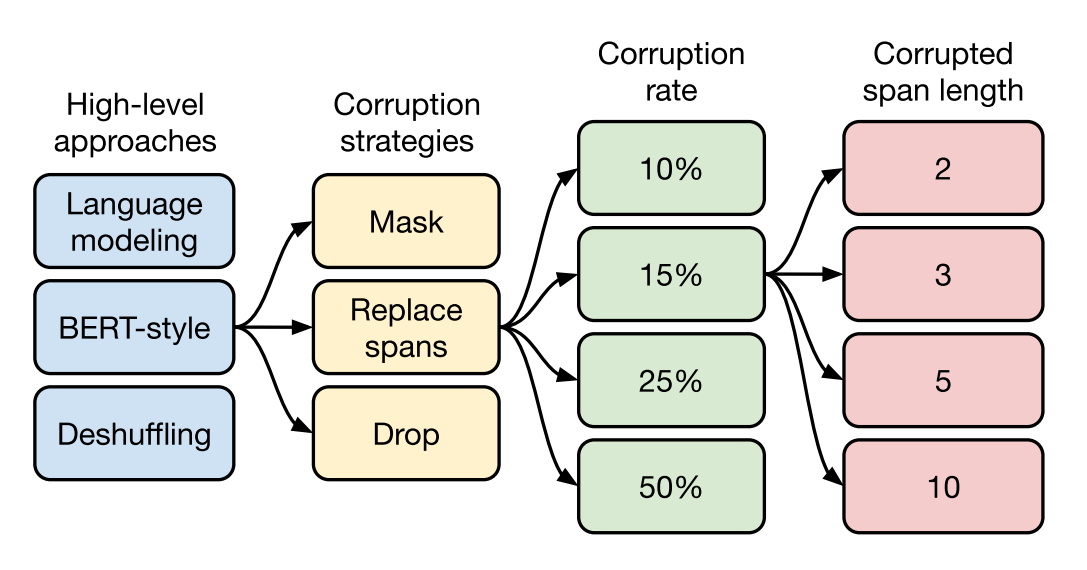
\includegraphics[width = 11cm]{figure/63-t5-objectives2.png}\\ 
		\citebutton{Source: Raffel et al., 2020}{https://jmlr.org/papers/v21/20-074.html}
	\end{figure}
	
\vfill

\end{frame}

% ------------------------------------------------------------------------------

\begin{frame}{The \textbf{C}olossal \textbf{C}lean \textbf{C}rawled \textbf{C}orpus (C4)}

\vfill

	\begin{itemize}
		\item Effort to measure the effect of quality, characteristics \& size of the pre-training resources
		\item Common Crawl as basis, careful cleaning and filtering for English language
		\item Orders of magnitude larger (750GB) compared to commonly used corpora 
	\end{itemize}
	
\vfill

\end{frame}

% ------------------------------------------------------------------------------

\begin{frame}{The \textbf{C}olossal \textbf{C}lean \textbf{C}rawled \textbf{C}orpus (C4)}

\vfill
	
	\textbf{Experiments (with respect to C4)}
	
	\begin{figure}
		\centering
		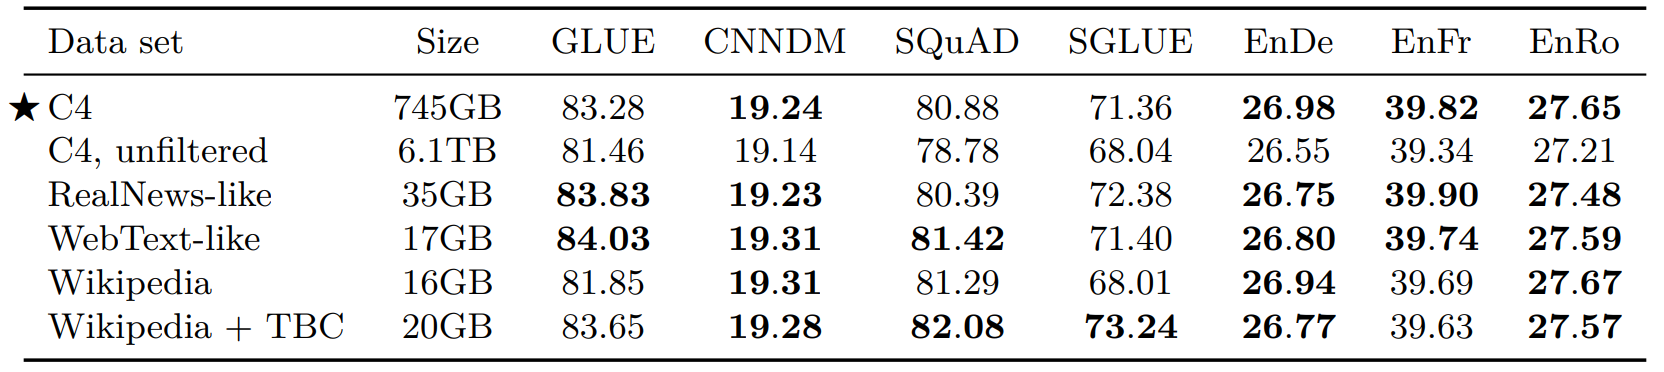
\includegraphics[width = 9cm]{figure/63-c4-characteristics.png}\\ 
		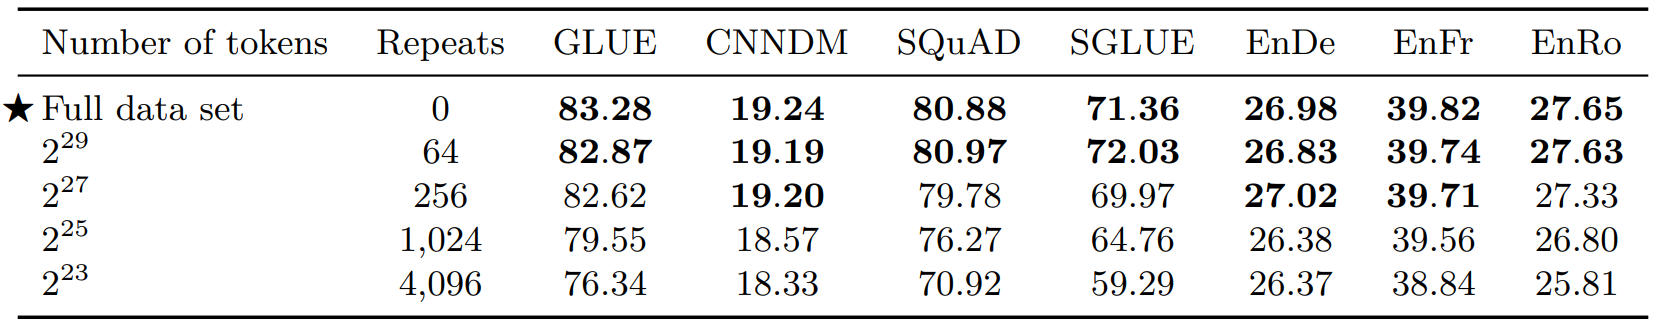
\includegraphics[width = 9cm]{figure/63-c4-size.png}\\ 
		\citebutton{Source: Raffel et al., 2020}{https://jmlr.org/papers/v21/20-074.html}
	\end{figure}
	
\vfill

\end{frame}

% ------------------------------------------------------------------------------

\begin{frame}{T5 - Exhaustive Experiments}

\vfill

	\textbf{Performed experiments with respect to ..}
	
	\begin{itemize}
		\item \textit{.. architecture, size \& objective}
		\item[$\to$] enc, dec, enc-dec
		\item[$\to$] Between 60M and 11B parameters
		\item \textit{.. details of the Denoising objective (which was found to work best)}
		\item \textit{.. fine-tuning methods}
		\item[$\to$] Adapter layers
		\item[$\to$] Gradual Unfreezing (cf. ULMFiT)
		\item \textit{.. Multi-task learning strategies}
		\item[$\to$] Examples-proportional mixing
		\item[$\to$] Temperature-scaled mixing
	\end{itemize}
	
\vfill

\end{frame}

% ------------------------------------------------------------------------------

\begin{frame}{Benchmark results}

\vfill

	\begin{figure}
		\centering
		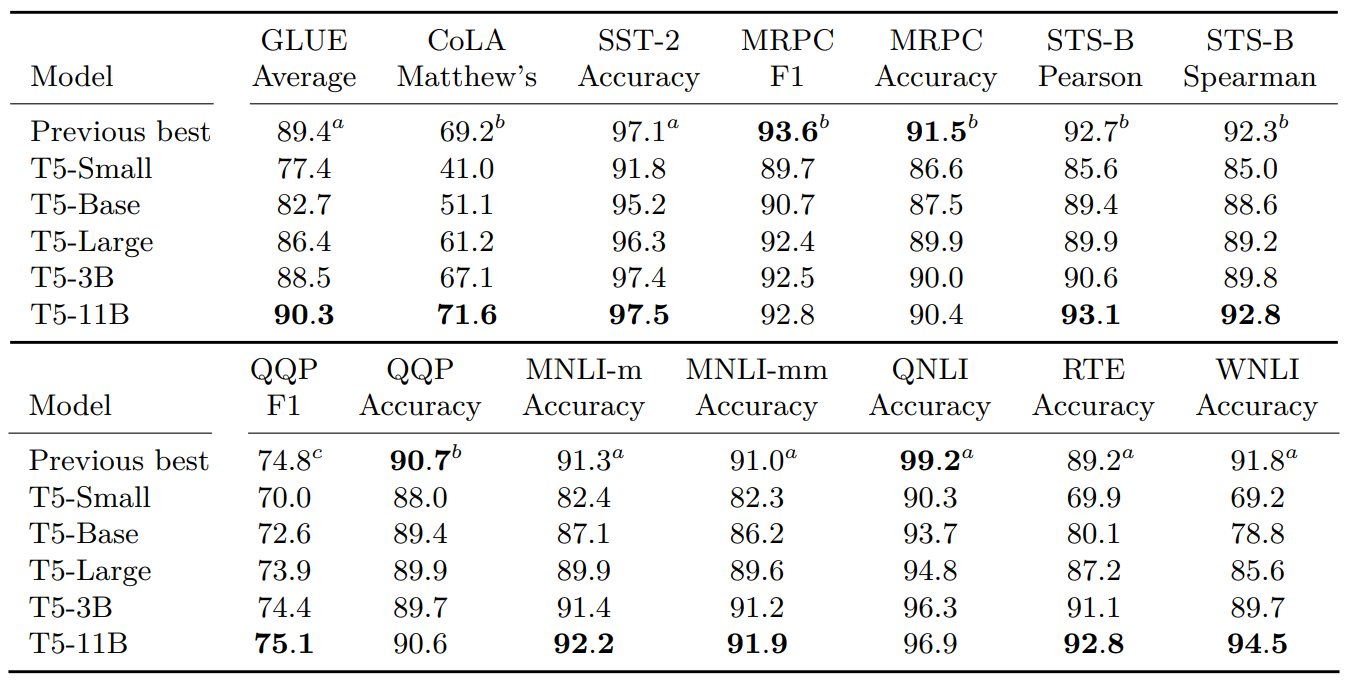
\includegraphics[width = 9cm]{figure/63-t5-glue.png}\\ 
		\citebutton{Source: Raffel et al., 2020}{https://jmlr.org/papers/v21/20-074.html}
	\end{figure}
	
\vfill

\end{frame}

% ------------------------------------------------------------------------------

\begin{frame}{Benchmark results}

\vfill

	\begin{figure}
		\centering
		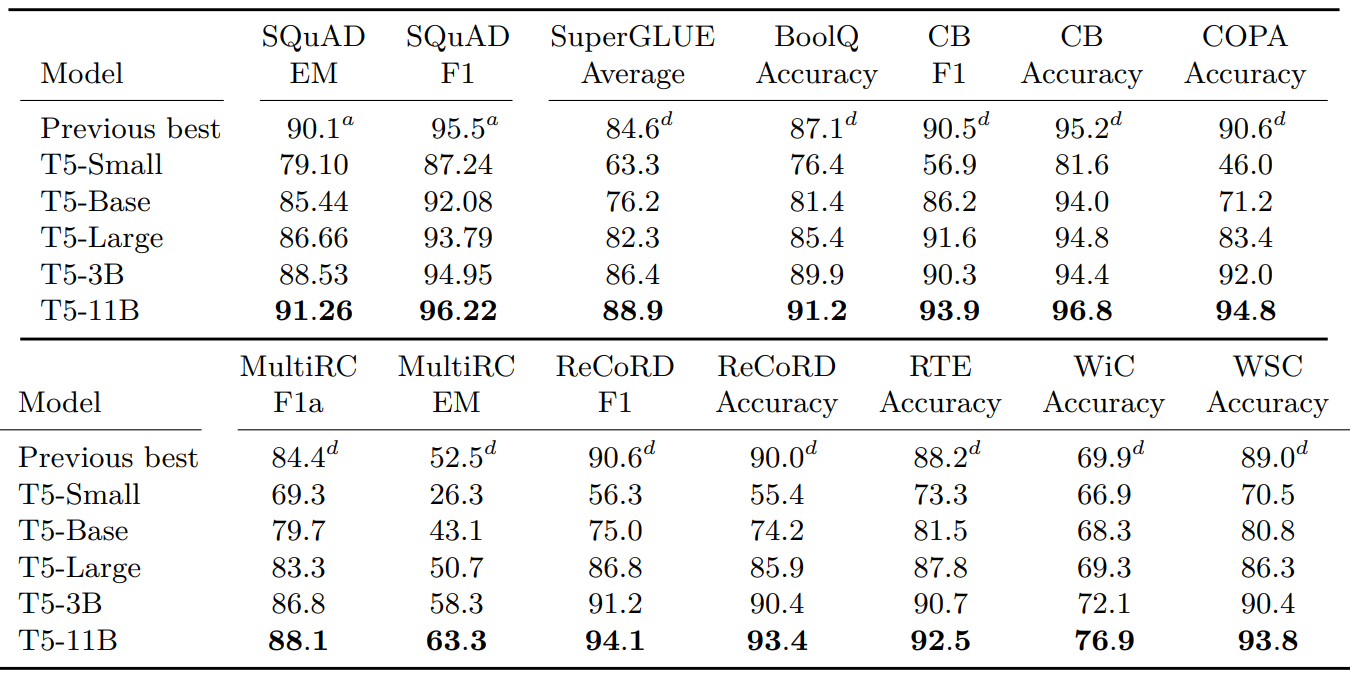
\includegraphics[width = 9cm]{figure/63-t5-squad-sglue.png}\\ 
		\citebutton{Source: Raffel et al., 2020}{https://jmlr.org/papers/v21/20-074.html}
	\end{figure}
	
\vfill

\end{frame}

% ------------------------------------------------------------------------------

\begin{frame}{Benchmark results}

\vfill

	\begin{figure}
		\centering
		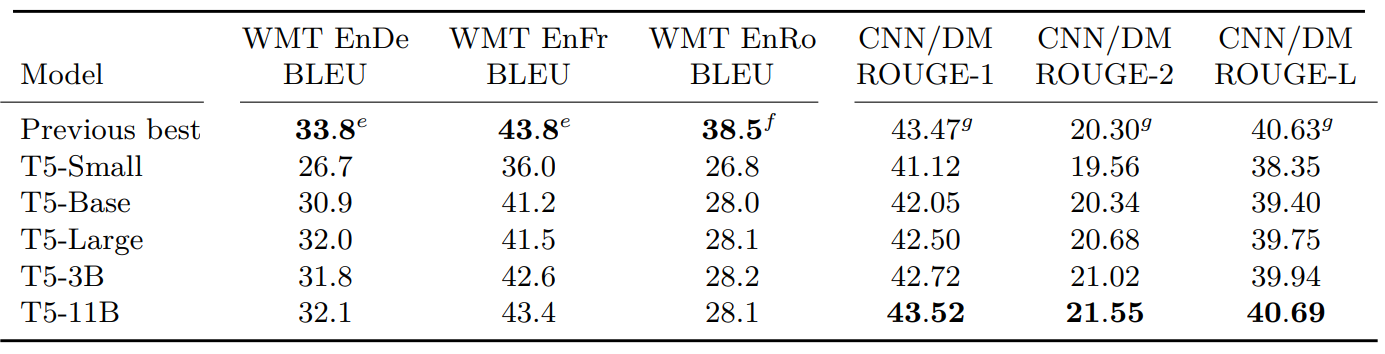
\includegraphics[width = 9cm]{figure/63-t5-mt.png}\\ 
		\citebutton{Source: Raffel et al., 2020}{https://jmlr.org/papers/v21/20-074.html}
	\end{figure}
	
\vfill

\end{frame}

% ------------------------------------------------------------------------------

\begin{frame}{T5 - Exhaustive Experiments}

\vfill
	
	\textbf{Conclusions}
	
	\begin{itemize}
		\item Encoder-decoder architecture works best in this "text-to-text" setting
		\item More data, larger models \& ensembling all boost the performance
			\begin{itemize}
				\item Larger models trained for fewer steps better than smaller models on more data
				\item Ensembling: Using same base pre-trained models worse than complete separate model ensembles
			\end{itemize}
		\item Different denoising objectives work similarly well
		\item Updating \textit{all} model parameters during fine-tuning works best (but expensive)
	\end{itemize}
	
\vfill

\end{frame}

% ------------------------------------------------------------------------------

\begin{frame}{Different T5 versions}
	\textit{Similar to BERT T5 has different versions, which all have a different parameter count} \citebutton{Raffel et al., 2020}{https://arxiv.org/abs/1910.10683}
	
	\hspace{}
	
	\begin{table}[h!]
	\centering
	\small % Reduce font size
	\begin{tabular}{|c|c|c|c|c|c|c|}
	\hline
	\textbf{Model} & \textbf{Parameters} & $\bm{n_{layers}}$ & $\bm{d_{model}}$ & $\bm{d_{FFN}}$ & $\bm{d_{qkv}}$ & $\bm{n_{heads}}$ \\ \hline
	small  & 60M  & 6  & 512  & 2048 & 64 & 8 \\ \hline
	base   & 220M & 12 & 768  & 3072 & 64 & 12 \\ \hline
	large  & 770M & 24 & 1024 & 4096 & 64 & 16 \\ \hline
	3B     & 3B   & 24 & 1024 & 16384 & 128 & 32 \\ \hline
	11B    & 11B  & 24 & 1024 & 65536 & 128 & 128 \\ \hline
	\end{tabular}
	\end{table}
	
	\begin{itemize}
		\item For T5 small, base and large we have the following parameter count per encoder/decoder layer:
		\begin{itemize}
			\item $N_{Encoder} = 12\cdot d_{model}^2$
			\item $N_{Decoder} = 16\cdot d_{model}^2$
		\end{itemize}
	\end{itemize}
	
	\hspace{}
	
	\textit{For T5 3B and 11B $N_{Encoder}$ and $N_{Decoder}$ are different!}
		
	\end{frame}
	
	
	
	%-------------------------------------------------------------------------------
	
	\begin{frame}{Approximate Parameter Count (1)}
	\textit{The general formula is:} $$N_{Total} = n_{layers}\cdot (N_{Encoder} + N_{Decoder}) + N_{Embedding}$$
	
	\begin{itemize}
		\item Let $V = 32000$ be the size of the vocabulary, we then have: $$N_{Embedding} = 32000 \times d_{model}$$
	
		\item \textbf{T5 small}:
			$$N_{small} = 6\cdot (12\cdot 512^2 + 16\cdot 512^2) + 32000\times 512 = 60,424,192$$
		\item \textbf{T5 base}:
			$$N_{base} = 12\cdot (12\cdot 768^2 + 16\cdot 768^2) + 32000\times 768 = 222,756,864$$
		\item \textbf{T5 large}:
			$$N_{large} = 24\cdot (12\cdot 1024^2 + 16\cdot 1024^2) + 32000\times 1024 = 737,411,072$$
		
	\end{itemize}
		
	\end{frame}
	
	%-------------------------------------------------------------------------------
	
	\begin{frame}{Revisiting: MHA and FFN (1)}
	
	\hspace{}
	
	\begin{itemize}
		\item In the transformer chapter we derived the FFN parameter count to be $\bm{8\cdot d_{model}}$
		\item We also derived the MHA parameter count to be $\bm{4\cdot d_{model^2}}$ 
		\item But this is only the case if we choose $d_{FFN} = 4\cdot d_{model}$ and $d_{qkv} = \frac{d_{model}}{n_{heads}}$, with $d_{FFN}$ being the hidden dimension of the FFN and $d_{qkv}$ being the embedding dimension of each head in MHA 
		\item For the two bigger model variants we have the following relations:
		\begin{itemize}
			\item \textbf{T5 3B}: $d_{FFN} = 16\cdot d_{model}$ and $d_{qkv} \neq \frac{d_{model}}{n_{heads}}$
			\item \textbf{T5 11B}: $d_{FFN} = 64\cdot d_{model}$ and $d_{qkv} \neq \frac{d_{model}}{n_{heads}}$ 
		\end{itemize}
		\item Thats why we can't use the same formulas as for the three previous variants
	\end{itemize}
		
	\end{frame}
	
	%-------------------------------------------------------------------------------
	
	\begin{frame}{Revisiting: MHA and FFN (2)}
	
	\begin{itemize}
		\item In MHA $n_{heads} \cdot d_{qkv}$ is no longer $d_{model}$:
	
	$$
	\begin{aligned}
	N_{attention} &= n_{heads} \cdot d_{qkv} \times d_{model} + (d_{model} \times d_{qkv}) \times n_{heads} \cdot 3 \\
	&= 4\cdot n_{heads}\cdot d_{qkv} \times d_{model}\text{;}\quad \text{instead of:}\quad 4\cdot d_{model}^2
	\end{aligned}
	$$
	
	\hspace{}
		
		\item For the FFN $d_{FFN}$ is no longer $4\cdot d_{model}$:
	
	$$    
	\begin{aligned}
	N_{FFN} &= d_{model} \times d_{FFN} + d_{FFN} \times d_{model} \\
	&= 2\cdot d_{model} \times d_{FFN}\text{;}\quad \text{instead of:}\quad 8\cdot d_{model}^2
	\end{aligned}
	$$
	
	\hspace{}
	
		\item For the Encoder and Decoder that means:
		\begin{itemize}
			\item $N_{Encoder} = 4\cdot n_{heads}\cdot d_{qkv} \times d_{model} + 2\cdot d_{model} \times d_{FFN}$
			\item $N_{Decoder} = 2\cdot 4\cdot n_{heads}\cdot d_{qkv} \times d_{model} + 2\cdot d_{model} \times d_{FFN} $
		\end{itemize}
	
	\end{itemize}
		
	\end{frame}
	
	%-------------------------------------------------------------------------------
	
	\begin{frame}{Approximate Parameter Count (2)}
	
	\textit{The general formula is still:} $$N_{Total} = n_{layers}\cdot (N_{Encoder} + N_{Decoder}) + N_{Embedding}$$
	
	\begin{itemize}
		\item \textbf{T5 3B}: 
	
		$$
		\begin{aligned}
			N_{3B} &= 24\cdot ([4\cdot 32\cdot 128 \times 1024 + 2\cdot 1024 \times 16384] \\
			&+ [2\cdot 4 \cdot 32\cdot 128 \times 1024 + 2\cdot 1024 \times 16384]) + 32000\cdot 1024 \\
			&= 2,851,340,288 \approx 3B
		\end{aligned}
		$$
	
		\hspace{}
	
		\item \textbf{T5 11B}:
		$$
		\begin{aligned}
			N_{11B} &= 24\cdot ([4\cdot 128\cdot 128 \times 1024 + 2\cdot 1024 \times 65536] \\
			&+ [2\cdot 4 \cdot 128\cdot 128 \times 1024 + 2\cdot 1024 \times 65536]) + 32000\cdot 1024 \\
			&= 11,307,057,152 \approx 11B
		\end{aligned}
		$$
	\end{itemize}
		
	\end{frame}
	
	%-------------------------------------------------------------------------------

\endlecture
\end{document}
